\documentclass[]{article}
\usepackage{authblk}
\usepackage{hyperref}
\usepackage{graphicx}
\usepackage{float}

\begin{document}
\title{Progressive File Transfer (PFT) Protocol}
\author{
	Jakob Buchgraber
	}

\maketitle
\tableofcontents
\newpage

\begin{abstract}
The progressive file transfer protocol (PFT) is a UDP-based protocol
that was developed for fast file transfers between a client and a
server. It supports both uploads and downloads, as well as pause
and restart of file transfers. Additionally, the protocol offers
flow control.
\end{abstract}


\section{Framing}

The frames are encoded on the wire in a framing format as specified in figure~\ref{framing}.
A PFT frame consists of a fixed 7 octet header and a variable length payload. The first
two octets specify the length of the entire frame, that is of the header and the variable
length payload. The next octet specifies the type of the frame. The last four octets of
the header specify an identifier, which uniquely identifies a connection. The identifier
is a pseudo-random byte sequence that must be chosen by the server. Both a server and
client are free to drop any frame with an unknown identifier. The variable length payload
contains the data of the specific frame type.

\begin{figure}[H]
\centering
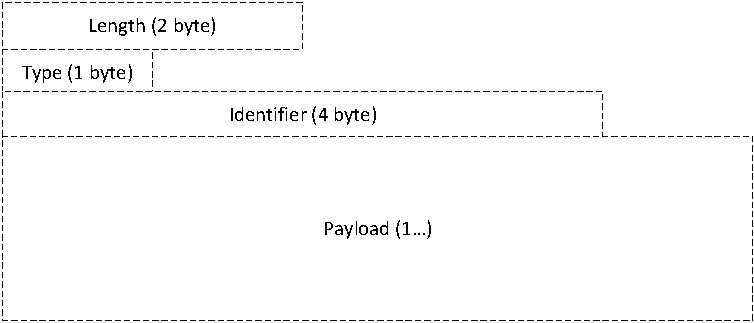
\includegraphics[width=\textwidth]{frames/framing.pdf}
\caption{Framing}
\label{framing}
\end{figure}

\section{Frames}

Subsequently we describe the format and semantics of all supported frame types. 

\subsection{Download Request}
\label{DOWNLOAD-REQ}

A client sends this frame to the server to initiate a new download
or resume a paused download. The identifier must always be set to zero.  
The SHA1 field is set to all zeroes in case of a new download, or to
the SHA1 hash of the whole file (as it exists on the server) 
in case of a paused download. The filename is a sequence of US ASCII
characters, where the last character must be followed by a zero octet.
Therefore, the protocol supports filenames of up to 255 octets in length.

\begin{figure}[H]
\centering
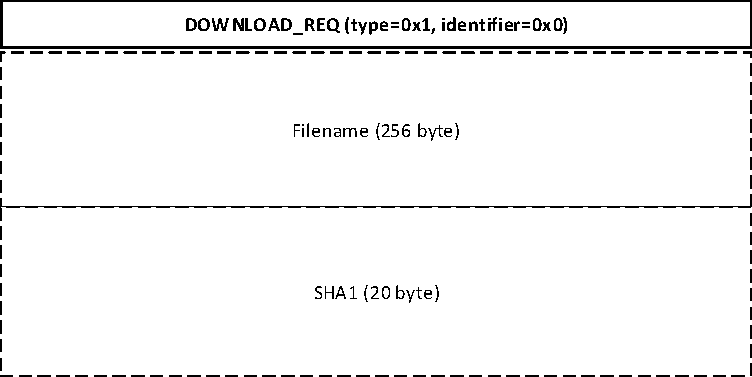
\includegraphics[width=\textwidth]{frames/download-req.pdf}
\caption{Download Request}

\end{figure}

\subsection{Download Response}

A server responds with this frame to a download request from the
client (Section~\ref{DOWNLOAD-REQ}). The frame has a random four 
byte identifier set, that uniquely identifies this download. All
future frames regarding this download (from both client and server)
must have this identifier set. A non-zero status indicates that the
download cannot be started. The detailed semantics of each status code are outlined
in the status code section (Section~\ref{STATUS-CODES}). The port field specifies to the client
on which server port to send any further frames for this download.
The port can either be the same as the port used to send the
download request to, or a new one. A server needs to make sure
that it can receive packets on the port before sending this frame. 
In case it doesn't receive any legal frames on this port within 30
seconds, it can stop listening and send a termination request (Section~\ref{TERMINATION-REQ})
with status code TIMEOUT to the client (using the same identifier).

\begin{figure}[H]
\centering
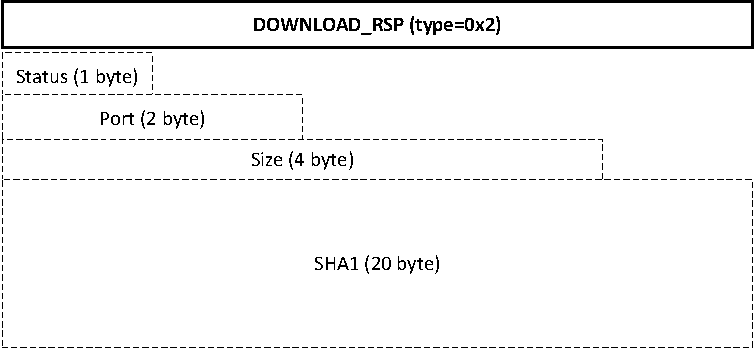
\includegraphics[width=\textwidth]{frames/download-rsp.pdf}
\caption{Download Response}
\label{DOWNLOAD-RSP}
\end{figure}

\subsection{Upload Request}

A client sends this frame to the server to initiate a new 
or resume a paused upload. The identifier must always be set to zero.  
The filename is a sequence of US ASCII
characters, where the last character must be followed by a zero octet.
Therefore, the protocol supports filenames of up to 255 octets in length.
The size field is an unsigned integer and must be set to the number
of bytes of the whole file. The SHA1 field must be set to the SHA1
of the whole file as well. So the upload request is identical for
new and paused uploads.

\begin{figure}[H]
\centering
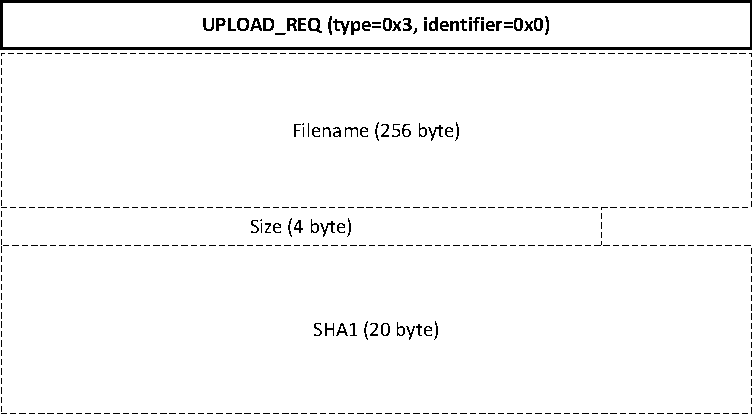
\includegraphics[width=\textwidth]{frames/upload-req.pdf}
\caption{Upload Request}
\label{UPLOAD-REQ}
\end{figure}

\subsection{Upload Response}

A server responds with this frame to an upload request from the
client (Section~\ref{UPLOAD-REQ}). The frame has a random four 
byte identifier set, that uniquely identifies an upload. All
future frames regarding a specific upload (from both client and server)
must have this identifier set. A non-zero status indicates that the
upload cannot be started. The detailed semantics of each status code are outlined
in the status code section. The port field specifies to the client
on which server port to send any further frames for this upload.
The port can either be the same as the port used to send the
upload request to, or a new one. A server needs to make sure
that it can receive packets on the port before sending this frame. 
In case it doesn't receive any legal frames on this port within 30
seconds, it can stop listening and send a termination request (Section~\ref{TERMINATION-REQ})
with status code TIMEOUT to the client (using the same identifier).

\begin{figure}[H]
\centering
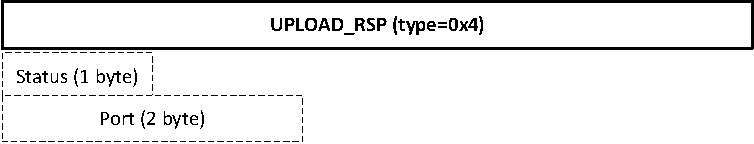
\includegraphics[width=\textwidth]{frames/upload-rsp.pdf}
\caption{Upload Response}
\label{UPLOAD-RSP}
\end{figure}

\subsection{Data Request}

This frame allows a local endpoint to request a sequence of bytes of
a given length at a specific byte offset in a file from a remote endpoint.
In case of a download the client sends this frame to the server, 
and in case of an upload the server sends this
frame to the client. Additionally, this frame also acts as an inbound
flow control mechanism for the data receiving side, as it specifies
exactly how much data an endpoint is ready to receive. An endpoint
must not send a data request frame, until all data requested by a 
previous data request frame have been received. 

\begin{figure}[H]
\centering
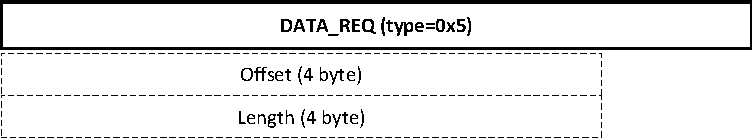
\includegraphics[width=\textwidth]{frames/data-req.pdf}
\caption{Data Request}
\label{DATA-REQ}
\end{figure}

\subsection{Data Response}

A data response frame may only be sent in response to a data request frame and
contains a sequence of bytes. It contains an offset and a length that uniquely identifies the byte sequence
within a file. That way, the order in which data response frames are received doesn't matter
, which is an important aspect as the underlying UDP transport doesn't gurantee order.

Depending on the network environment, a data request frame can be answered by multiple
data response frames. That is, a receiving endpoint might request one megabyte of data, but
due to packet size limitations the sending endpoint may respond with 250 data response
frames each carrying four kilobytes of data.
 
\begin{figure}[H]
\centering
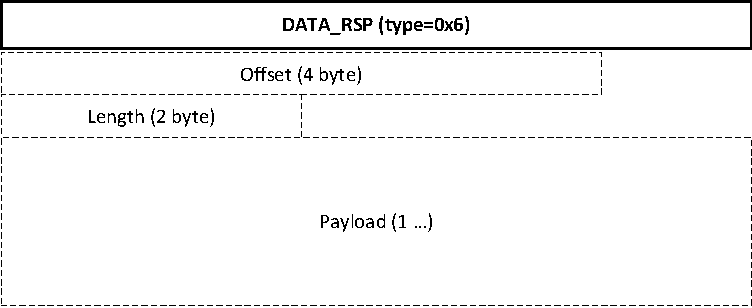
\includegraphics[width=\textwidth]{frames/data-rsp.pdf}
\caption{Data Response}
\label{DATA-RSP}
\end{figure}

\subsection{Checksum Request}
A checksum request frame may only be sent by the data receiving side. That is, by the client
in case of a download or by the server when uploading. It's used to verify the checksum of
the whole file or a part of it. It's intended to be sent after having fully received
the data of a data request, and allows the receiving side to verify the correctness early
on, as opposed to after the download or upload has finished. It may also be used to verify 
the correctness of a partially down- or uploaded file, immediately after having restarted
a down- or upload. 

\begin{figure}[H]
\centering
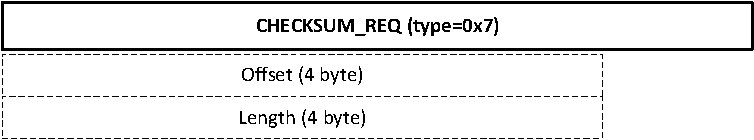
\includegraphics[width=\textwidth]{frames/checksum-req.pdf}
\caption{Checksum Request}
\label{CHECKSUM-REQ}
\end{figure}

\subsection{Checksum Response}
A checksum response frame is sent in response to a checksum request frame. It contains the SHA1
hash of the length bytes at offset. 

\begin{figure}[H]
\centering
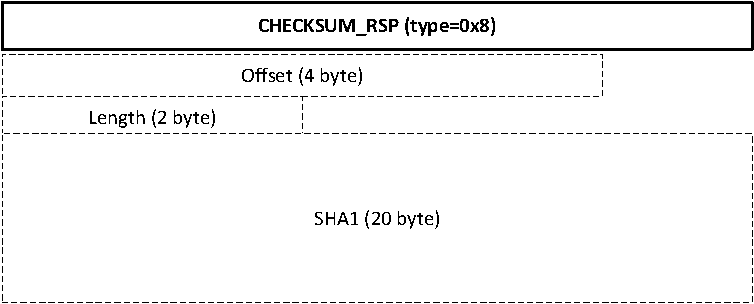
\includegraphics[width=\textwidth]{frames/checksum-rsp.pdf}
\caption{Checksum Response}
\label{CHECKSUM-RSP}
\end{figure}

\subsection{Termination Request}
\label{TERMINATION-REQ}

This frame can be send by either side of an upload and
download and at any point in time. After receiving
a termination request frame an endpoint needs to make a best
effort to stop any communication for the given identifier.
An endpoint is free to drop any frames received after having 
sent a termination request.

\begin{figure}[H]
\centering
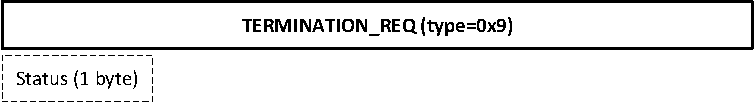
\includegraphics[width=\textwidth]{frames/shutdown-req.pdf}
\caption{Termination Request}

\end{figure}

\section{Status Codes}
\label{STATUS-CODES}

\begin{itemize}
\item[\textbf{OK (0x0)}] There were no errors and everything went as expected. 
\item[\textbf{ERROR (0x1)}] Something went wrong.
\item[\textbf{TIMEOUT (0x2)}] An upload or download timed out. The receiver is free to retry immediately.
\item[\textbf{RETRY (0x3)}] The download or upload should be retried a later point with a new upload or download request.
\end{itemize}

\newpage

\section{Example Download}
This interaction diagram shows how a client might download a 16KB text file from a server.

\begin{figure}[H]
\centering
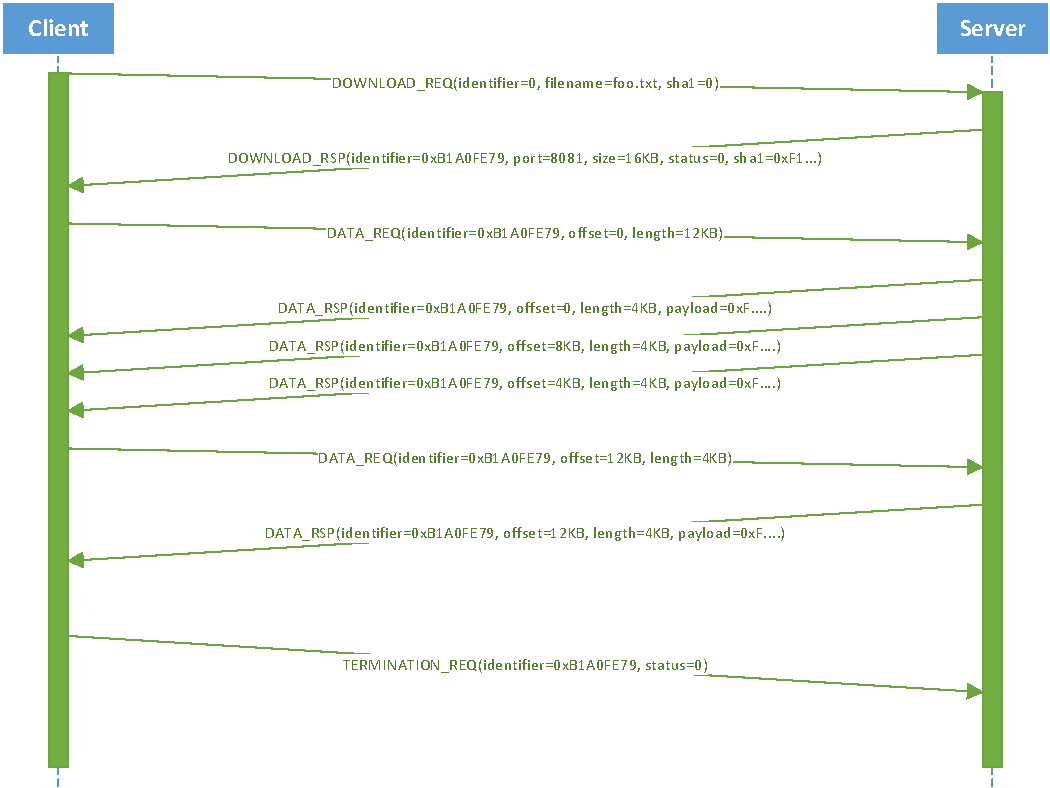
\includegraphics[width=\textwidth]{frames/download-interaction.pdf}
\caption{Example Download}
\label{EXAMPLE-DOWNLOAD}
\end{figure}


\end{document}
